\documentclass{standalone}
\usepackage{pgfplots}
\usepackage{tikz}
\pgfplotsset{compat=1.18}

\begin{document}
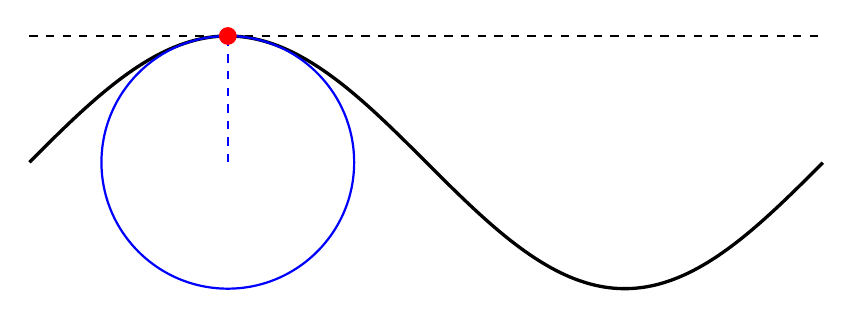
\begin{tikzpicture}
\begin{axis}[
    axis lines=none,
    xmin=0, xmax=6.28,
    ymin=-2, ymax=2,
    axis equal,
    width=12cm,
    height=8cm,
]

% Define the sine curve from 0 to 2π
\addplot[
    domain=0:6.28,
    samples=200,
    very thick,
    black
] {sin(deg(x))};

% Point of interest: (π/2, 1) - the crest of the sine wave
% Mark the point at the crest
\addplot[only marks, mark=*, mark size=3pt, red] coordinates {(1.5708, 1)};

% Tangent line at the crest (horizontal line)
\addplot[
    domain=0:6.28,
    thick,
    black,
    dashed
] {1};

% Osculating circle with center at (π/2, 0) and radius 1
\coordinate (center) at (1.5708, 0);
\draw[thick, blue] (center) circle [radius=1];

% Draw radius of osculating circle in dashed blue
\draw[thick, blue, dashed] (1.5708, 0) -- (1.5708, 1);

\end{axis}
\end{tikzpicture}
\end{document}
